\documentclass[12pt, a4paper]{article}
\usepackage{caption}
\usepackage{graphicx}
\usepackage{hyperref}
\usepackage{relsize}
\hypersetup{
    colorlinks,
    citecolor=black,
    filecolor=black,
    linkcolor=black,
    urlcolor=black
} 

\title{Computer Architecture\\Assignment 1}
\date{2022}
\author{Kristoffer Klokker}

\usepackage{xcolor,listings}
\usepackage{textcomp}
\usepackage{color}
\usepackage{listings}
\definecolor{codegreen}{rgb}{0,0.6,0}
\definecolor{codegray}{rgb}{0.5,0.5,0.5}
\definecolor{codepurple}{HTML}{C42043}
\definecolor{backcolour}{HTML}{F2F2F2}
\definecolor{bookColor}{cmyk}{0,0,0,0.90}  
\color{bookColor}

\lstset{upquote=true}

\lstdefinestyle{mystyle}{
    backgroundcolor=\color{backcolour},   
    commentstyle=\color{codegreen},
    keywordstyle=\color{codepurple},
    stringstyle=\color{codepurple},
    basicstyle=\footnotesize\ttfamily,
    breakatwhitespace=false,
    breaklines=false,
    captionpos=b,
    keepspaces=true,
    numbers=left,
    numbersep=10pt,
    showspaces=false,
    showstringspaces=false,
    showtabs=false,
    tabsize=3,
	 morecomment = [l][\nullfont]{\#}
}


\lstset{style=mystyle}

\begin{document}
	\maketitle
	\clearpage
	\tableofcontents
	\clearpage
	\section{Introduction}
	The following report will cover, the implementation of different sorting algorithms in assembly x86 64 bit AT\&T flavor. Moreover will the implementations be benchmarked and compared to find the fastest algorithm. From the benchmark resulta conclusion will then be made, on choice of algorithm based on speed and implementation complexity.\\
	The sorting algorithms will be applied upon a set of coordinates, from which the sorting is based upon the $y$ coordinate. In the implementation the $x$ coordinate is not accounted for. Therefore coordinates may not be in the same order between algorithms.\\
	The coordinates is given in a file, which is given as argument to the sorter. The file consist of coordinates in the format:
	$$<y>\setminus t<x>\setminus n$$
	The $<x>$ and $<y>$ coordinate will be in the range of 0 to 32767 i.e. 16 bit format.\\
	The sorter then have to return the sorted coordinates in the same format using the stdout.
	\section{Design of implementation and test}
		To work with the sorting algorithms and comparing them, will they be implemented as independent functions. This will help in making the benchmarks more even and making the algorithm more true to their definition.\\
		To ensure combatibility the functions will take two paramters, a pointer to the start of the array and end of the array. 
	\section{Implementing Read, Parse \& Print}
		In order to implement and test sorting algorithms, first a reader, formatter and printer must be setup. This is done separately the sorting functions, such the comparisons are more equal and the implementation represent a general solution to a sorting function.
		\subsection{Read}
		To create the most consisting test environment for the sorting functions, is the reader implemented to read the whole file into memory. Therefore the reading of the file is done in the following steps:
			\begin{enumerate}
				\addtolength\itemsep{-2mm}
					  \item The file descriptor is obtained from the given argument using open system call
						\item The size of the file is found using fstat system call
						\item Space is allocated for the file by using sbrk to find the current data segment address and then using the file size find the new data segment end address and allocate space using sbrk
						\item The file is read into the allocated space using read system call
			\end{enumerate}
		\subsection{Parse and Format}
			When the data is read into memory, it will be in ascii format. To make the data easier to work with a parser is used to convert the ascii numbers into decimal.\\
			For converting a parser was implemented. The parser function takes an address to the start of the ascii number, and then first the $x$ value is converted by using a sum in the following way:
			\begin{enumerate}
				\addtolength\itemsep{-2mm}
				\item Multiply sum by 10
				\item Take next byte and subtract by 48 to convert from ascii to decimal
				\item Add decimal to sum
				\item Repeat until $\setminus t$ or $\setminus n$ is found
			\end{enumerate}
			This is then repeated to get the $y$ value.\\[4mm]
			The two coordinates is then returned, from which it can be used for sorting.\\
			To prevent having the convert for each comparison, the coordinates can be written into memory. By using the coordinate range limit, the coordinates $x$ and $y$ can be written into a 32 bit register. This therefore makes it possible to store a coordinate in 32 bits. This also makes it easier to work with since the spacing will be static.\\
			Instead of allocating more space for the coordinates, can the file content can be overwritten. This is possible since the minimum size for a file will be the file containing only two single digit coordinates. This file size will be 32 bit since the file contains 4 characters (2 digits, $\setminus n$ and $\setminus t$). Therefore the 32 bit coordinate can be written in the same space, making the need for more allocated space not necessary.
		\subsection{Print}
			With the 32 bit coordinate format, it is not possible to print directly from memory.\\
			First the coordinates $x$ and $y$ have to be converted back into ascii. This is done in the following way:
			\begin{enumerate}
				\addtolength\itemsep{-2mm}
				\item Create a divisor equal to 10000, since the values most significant digit is in the 10000 order.
				\item Get the most significant digit by digit by dividing with divisor
				\item Set value equal to remainder
				\item Add 48 to convert to ascii
				\item Add ascii value to print buffer
				\item Divide divisor by 10
				\item Repeat from step two until divisor is 0
			\end{enumerate}
			After this the print buffer is written into stdout. When the $x$ value is printed a $\setminus t$ is printed and likewise with $y$ a $\setminus n$ is printed.
	\section{Sorting algorithms}
		To sort the coordinates, the following algorithms was implemented.
		\begin{itemize}
				\addtolength\itemsep{-2mm}
			\item Insertion sort
			\item Quicksort
			\item Heap sort
		\end{itemize}
		Each algorithm is implemented as per definition, with only changes to step amounts to account for coordinate format. Each sorting function then took two arguments, a pointer to the start, and a pointer to the end of the array.
		\subsection{Insertion sort}
			Insertion sort was implemented using 2 nested loops.\\
			The first loop went from the start of the array to the end of the array, getting each coordinate $c_n$ which should be sorted.\\
			The second loop consisted of:
			\begin{enumerate}
				\addtolength\itemsep{-2mm}
				\item Exit loop if the start of the array is reached
				\item Exit loop if $c_{n-1} \leq c_n$ 
				\item Switch $c_{n-1}$ with $c_n$ 
				\item Repeat from step 1 using $c_{n-1}$
			\end{enumerate}
		\subsection{Quicksort}
			Quicksort was implemented using a main loop, which called itself recursively. The main loop consisted of:
			\begin{enumerate}
				\addtolength\itemsep{-2mm}
				\item Exit loop if the given array length is smaller or equal to 1
				\item Choose the first coordinate as sorting point
				\item sortArray loop
				\item Move chosen coordinate in between smaller and larger basket
				\item Call quicksort on smaller basket and larger basket
			\end{enumerate}
			The sortArray loop went through each coordinate and checked if the coordinates $y$ value was higher than the chosen $y$ coordinate. In the case of a higher value, the value is switched with the value at the large stack end pointer, and the large stack end pointer is incremented. 
		\subsection{Heap sort}
			Heap sort consisted of the main sorting function and the function maxHeapify.\\	
			The maxHeapify function is used to make the, array in a maximum heap order in the following manner:
			\begin{enumerate}
				\addtolength\itemsep{-2mm}
				\item Get references to right and left node
				\item Set largest value to root
				\item Set largest value to left if left is in the array and larger than root
				\item Set largest value to right if in array and larger than largest value
				\item If largest value is not root, switch largest value and root and call maxHeapify on switched node
			\end{enumerate}

			\begin{minipage}{0.4\textwidth}
				\lstinputlisting[firstline=3,lastline=34]{../src/sortingAlgo.s}
			\end{minipage}
			\begin{minipage}{0.6\textwidth}
				To explain heap sort, a code snippet is included, since the heap sort implmentation was the most convoluted to implment in assembly. The heap sort function implmeneted by:
				\begin{enumerate}
					\item Get a pointer to the lower middle of the array 2 - 6
					\item Ensure the middle is divisible by 4 such it points correctly to coordinates 7 - 13
					\item Go through each coordinate and init heap structure 14 - 20
					\item Move first element to end of array and shorten array 22 - 25
					\item Call maxHeapify on the first element 28
					\item Repeat heapLoop until every element is out of the array 29 - 32
				\end{enumerate}
 			\end{minipage}\\
			\section{Benchmarks}
		\subsection{Overhead}
			To find the overhead time, the sorting algorithm was not called. Therefore the overhead time measure included: Opening and reading file into memory, formatting file content, print formatted content in original format.
				\begin{figure}[h]
						  \centering
						  \includegraphics[width=240px]{assets/overhead.eps}
						  \caption{Graph over time in seconds as a function of number of coordinates}
							\label{fig:overhead}
				\end{figure}	
				As seen on the graph \ref{fig:overhead}, the growth is a linear relation to the file size. Since the relation is linear, the overhead time will have no influence on the overall run time, since the fastest sorting algorithm implemented runs in $O(n\log n)$.\\
			This is also reflected in the user time and system time. Using insertion sort the user time was on overage 100\% of the real time.
			This is not as clear in the quicksort and heap sort. Their lower run time made fluctuations more likely, but as the file size gets larger the user time should also begin to increase.
		\subsection{Fastest sorting algorithm}
		
			The benchmark results reflects the expected outcome.\\
			It can be seen in the graph \ref{fig:performance}, that insertion sorts run time has a faster grow time than quicksort and heap sort. Likewise is it seen that heap sort has a slight lower growth rate than quicksort. This likewise reflects quicksorts ability to run near $O(n\log n)$, but in worst case runs at $O(n^2)$.\\	
			\begin{figure}[h]
				\centering
				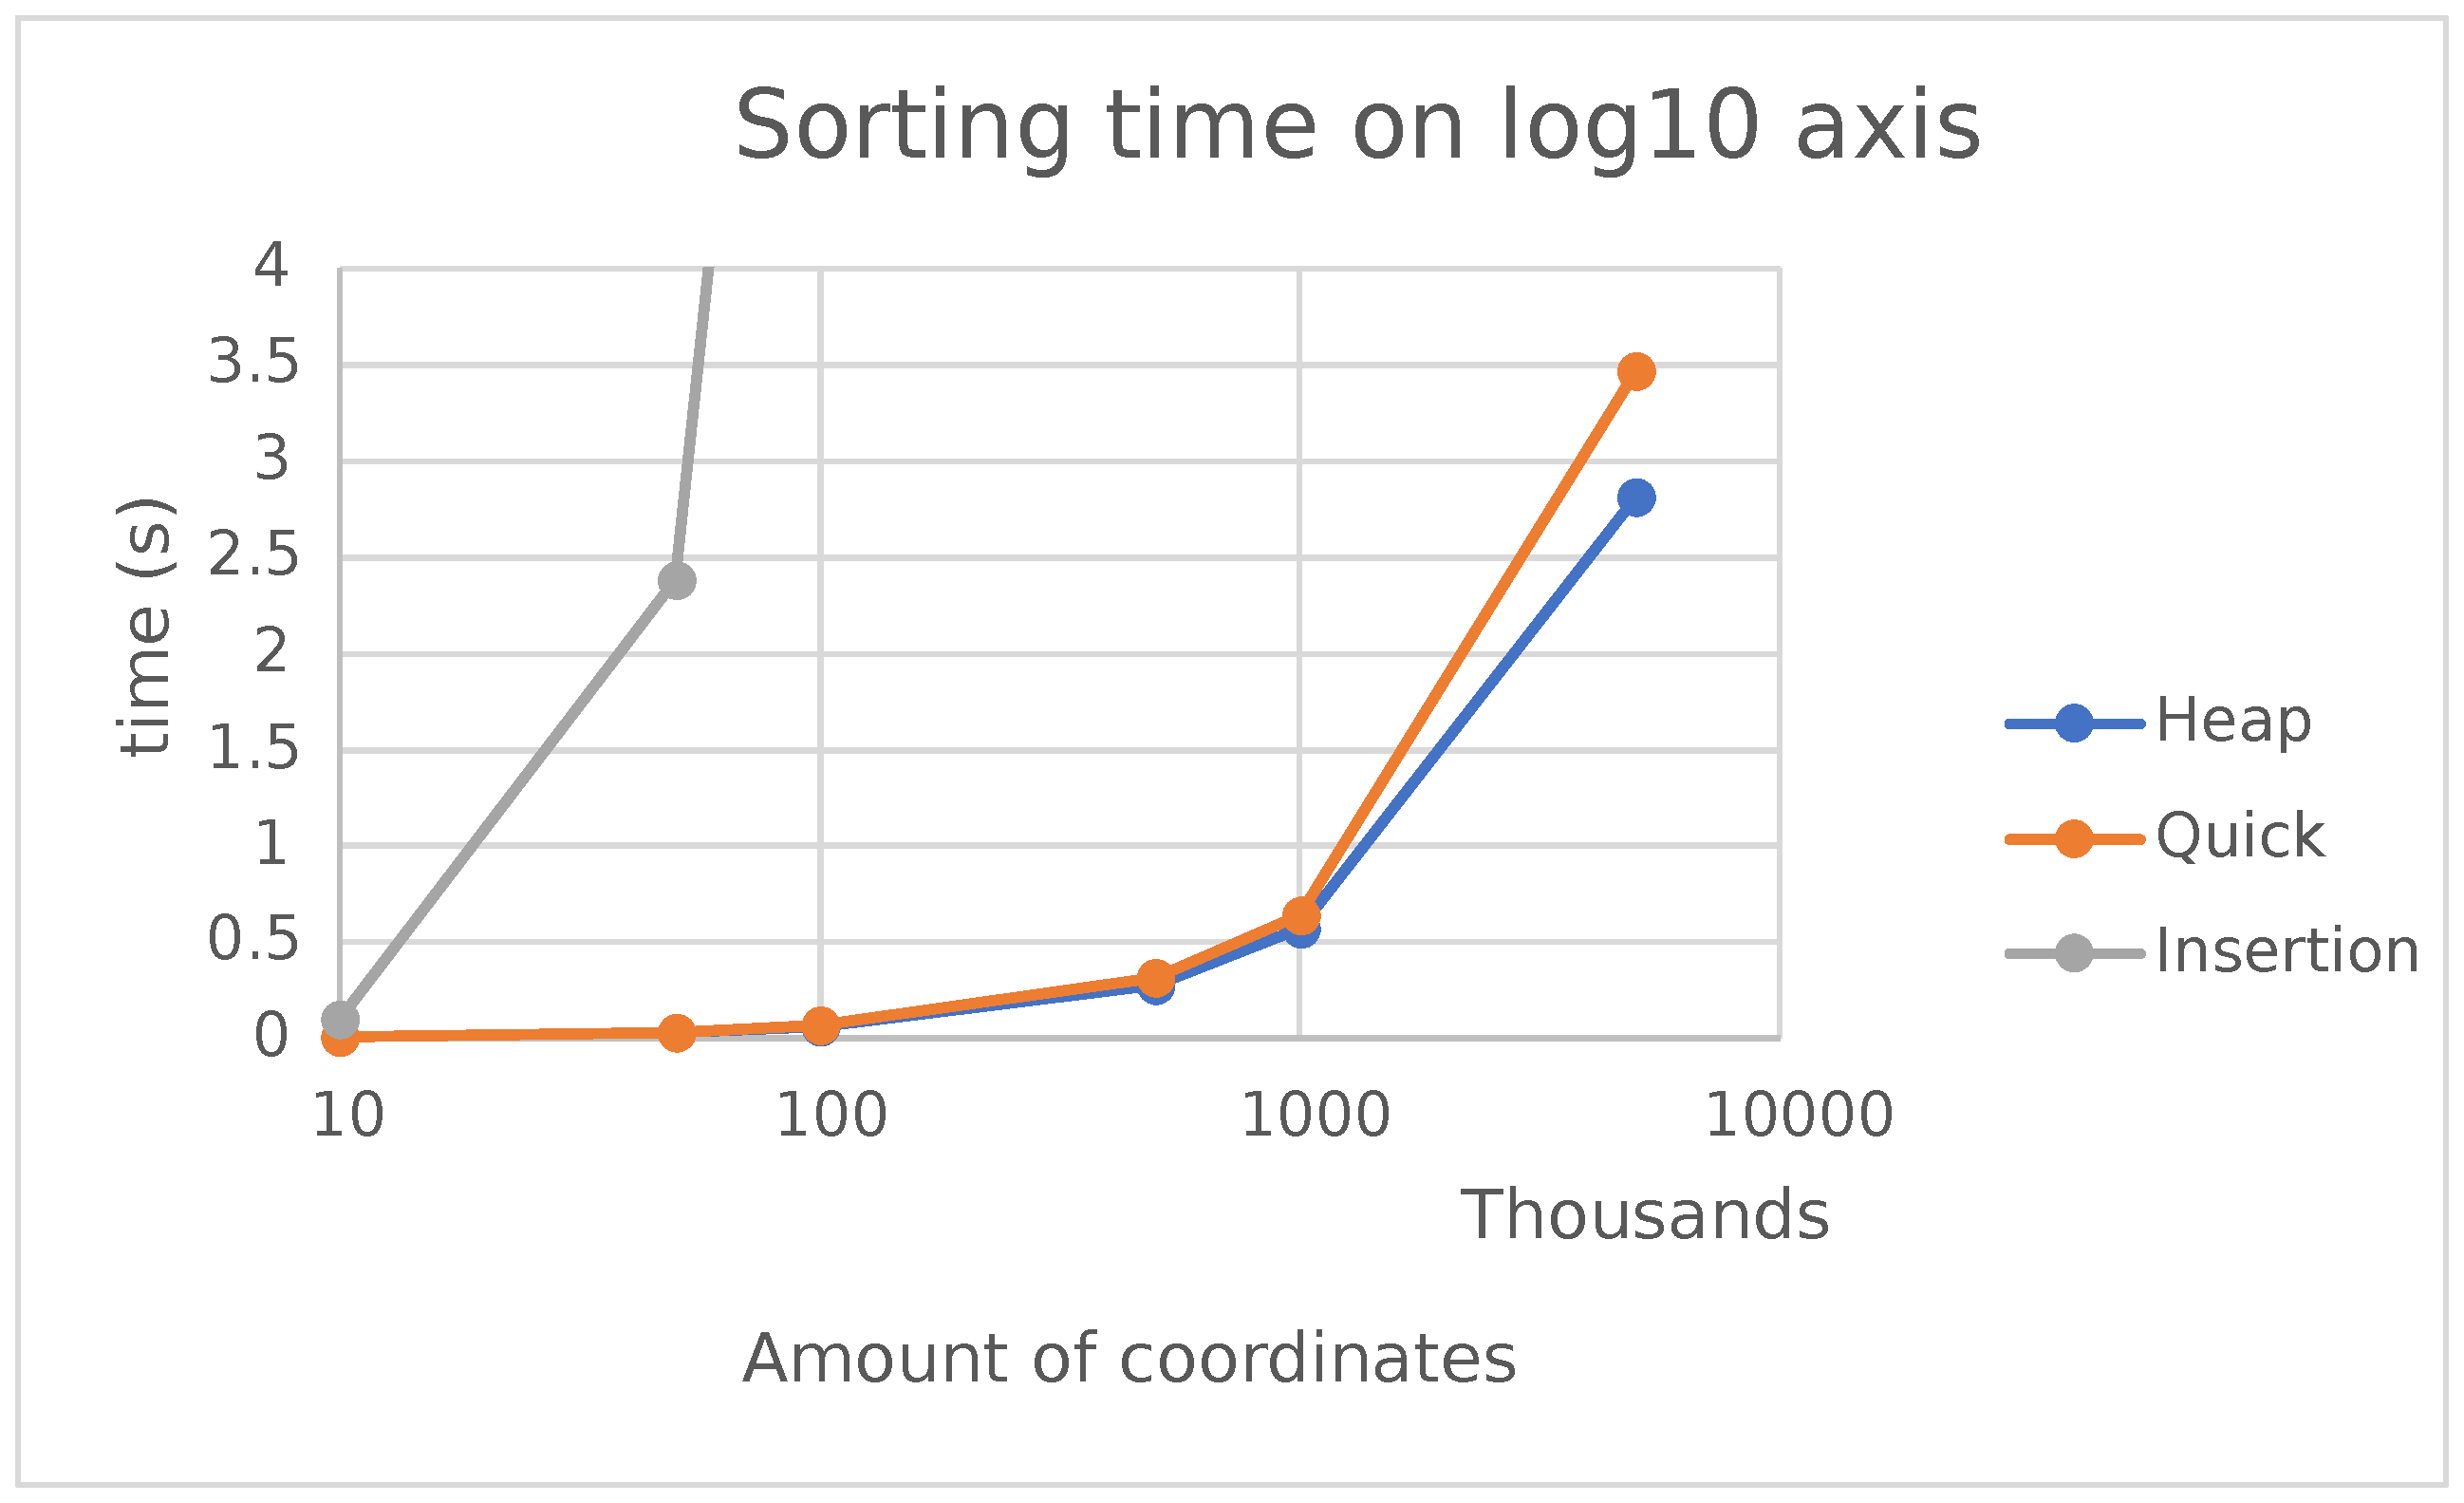
\includegraphics[width=275px]{assets/performance.eps}
				\caption{Graph over time in seconds as a function of number of coordinates for the three implemented sorting algorithms}
				\label{fig:performance}
			\end{figure}	
			\begin{figure}[h]
				\centering
				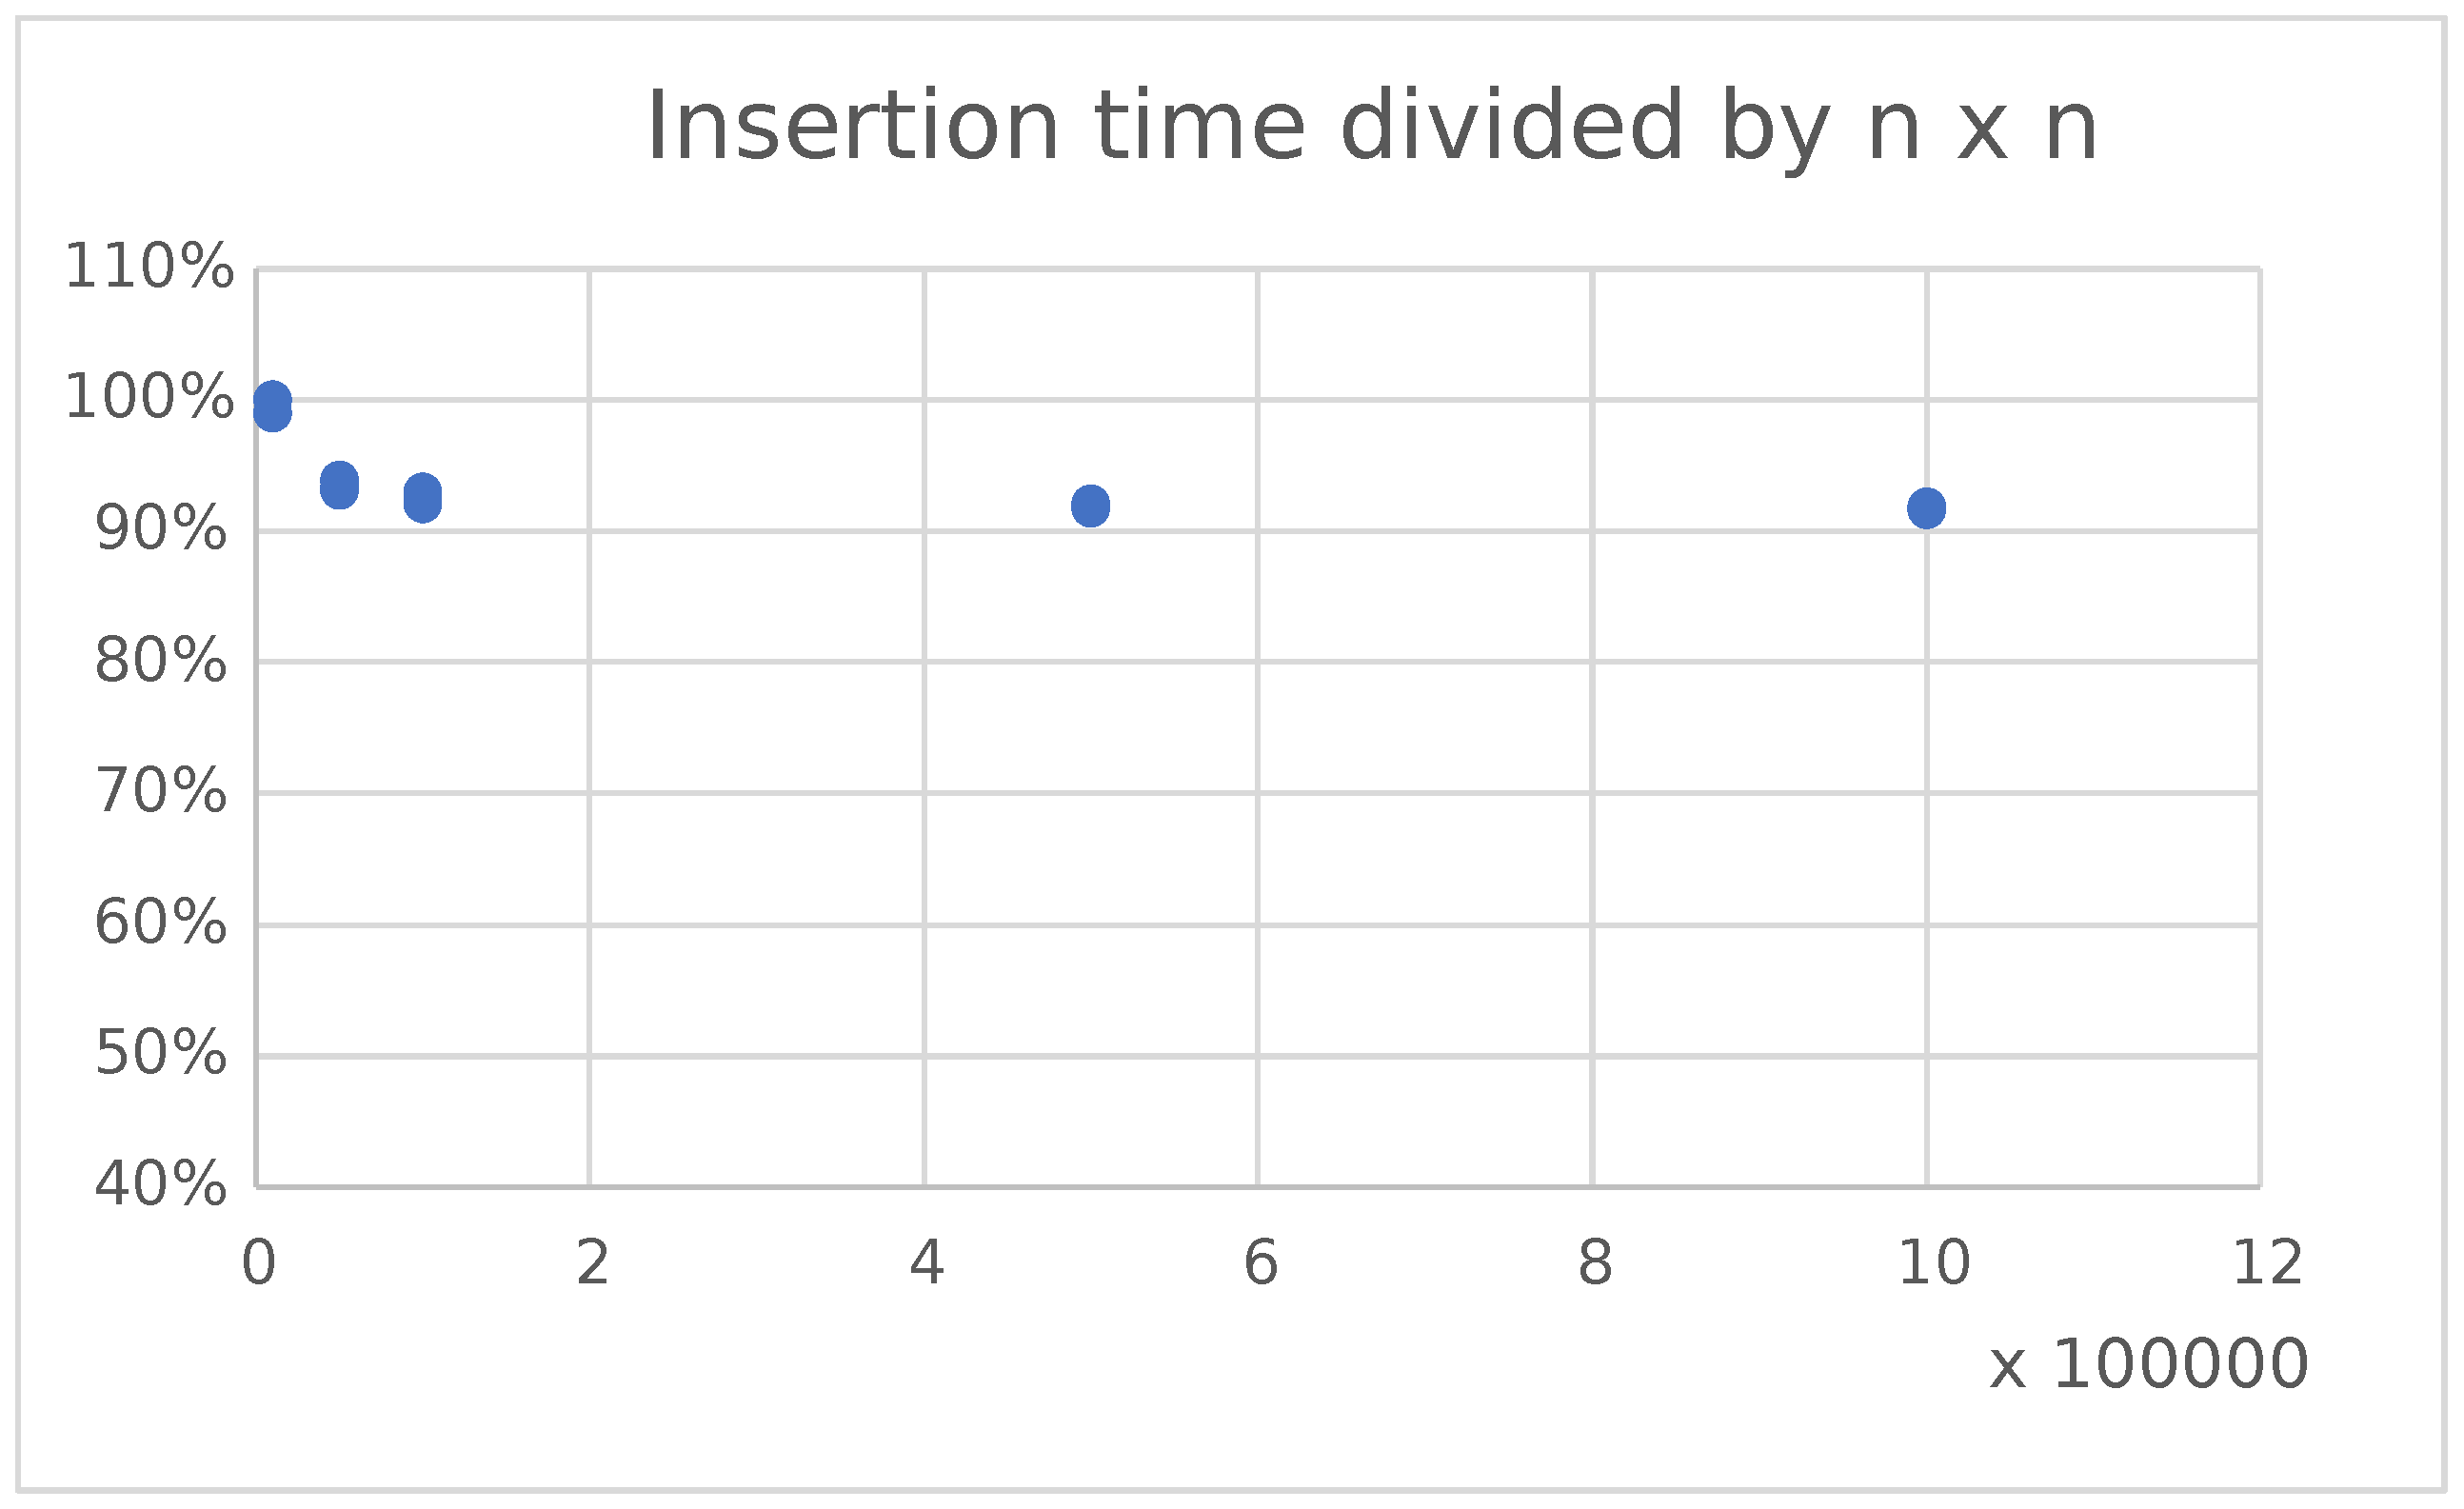
\includegraphics[width=185px]{assets/insertion.eps}
				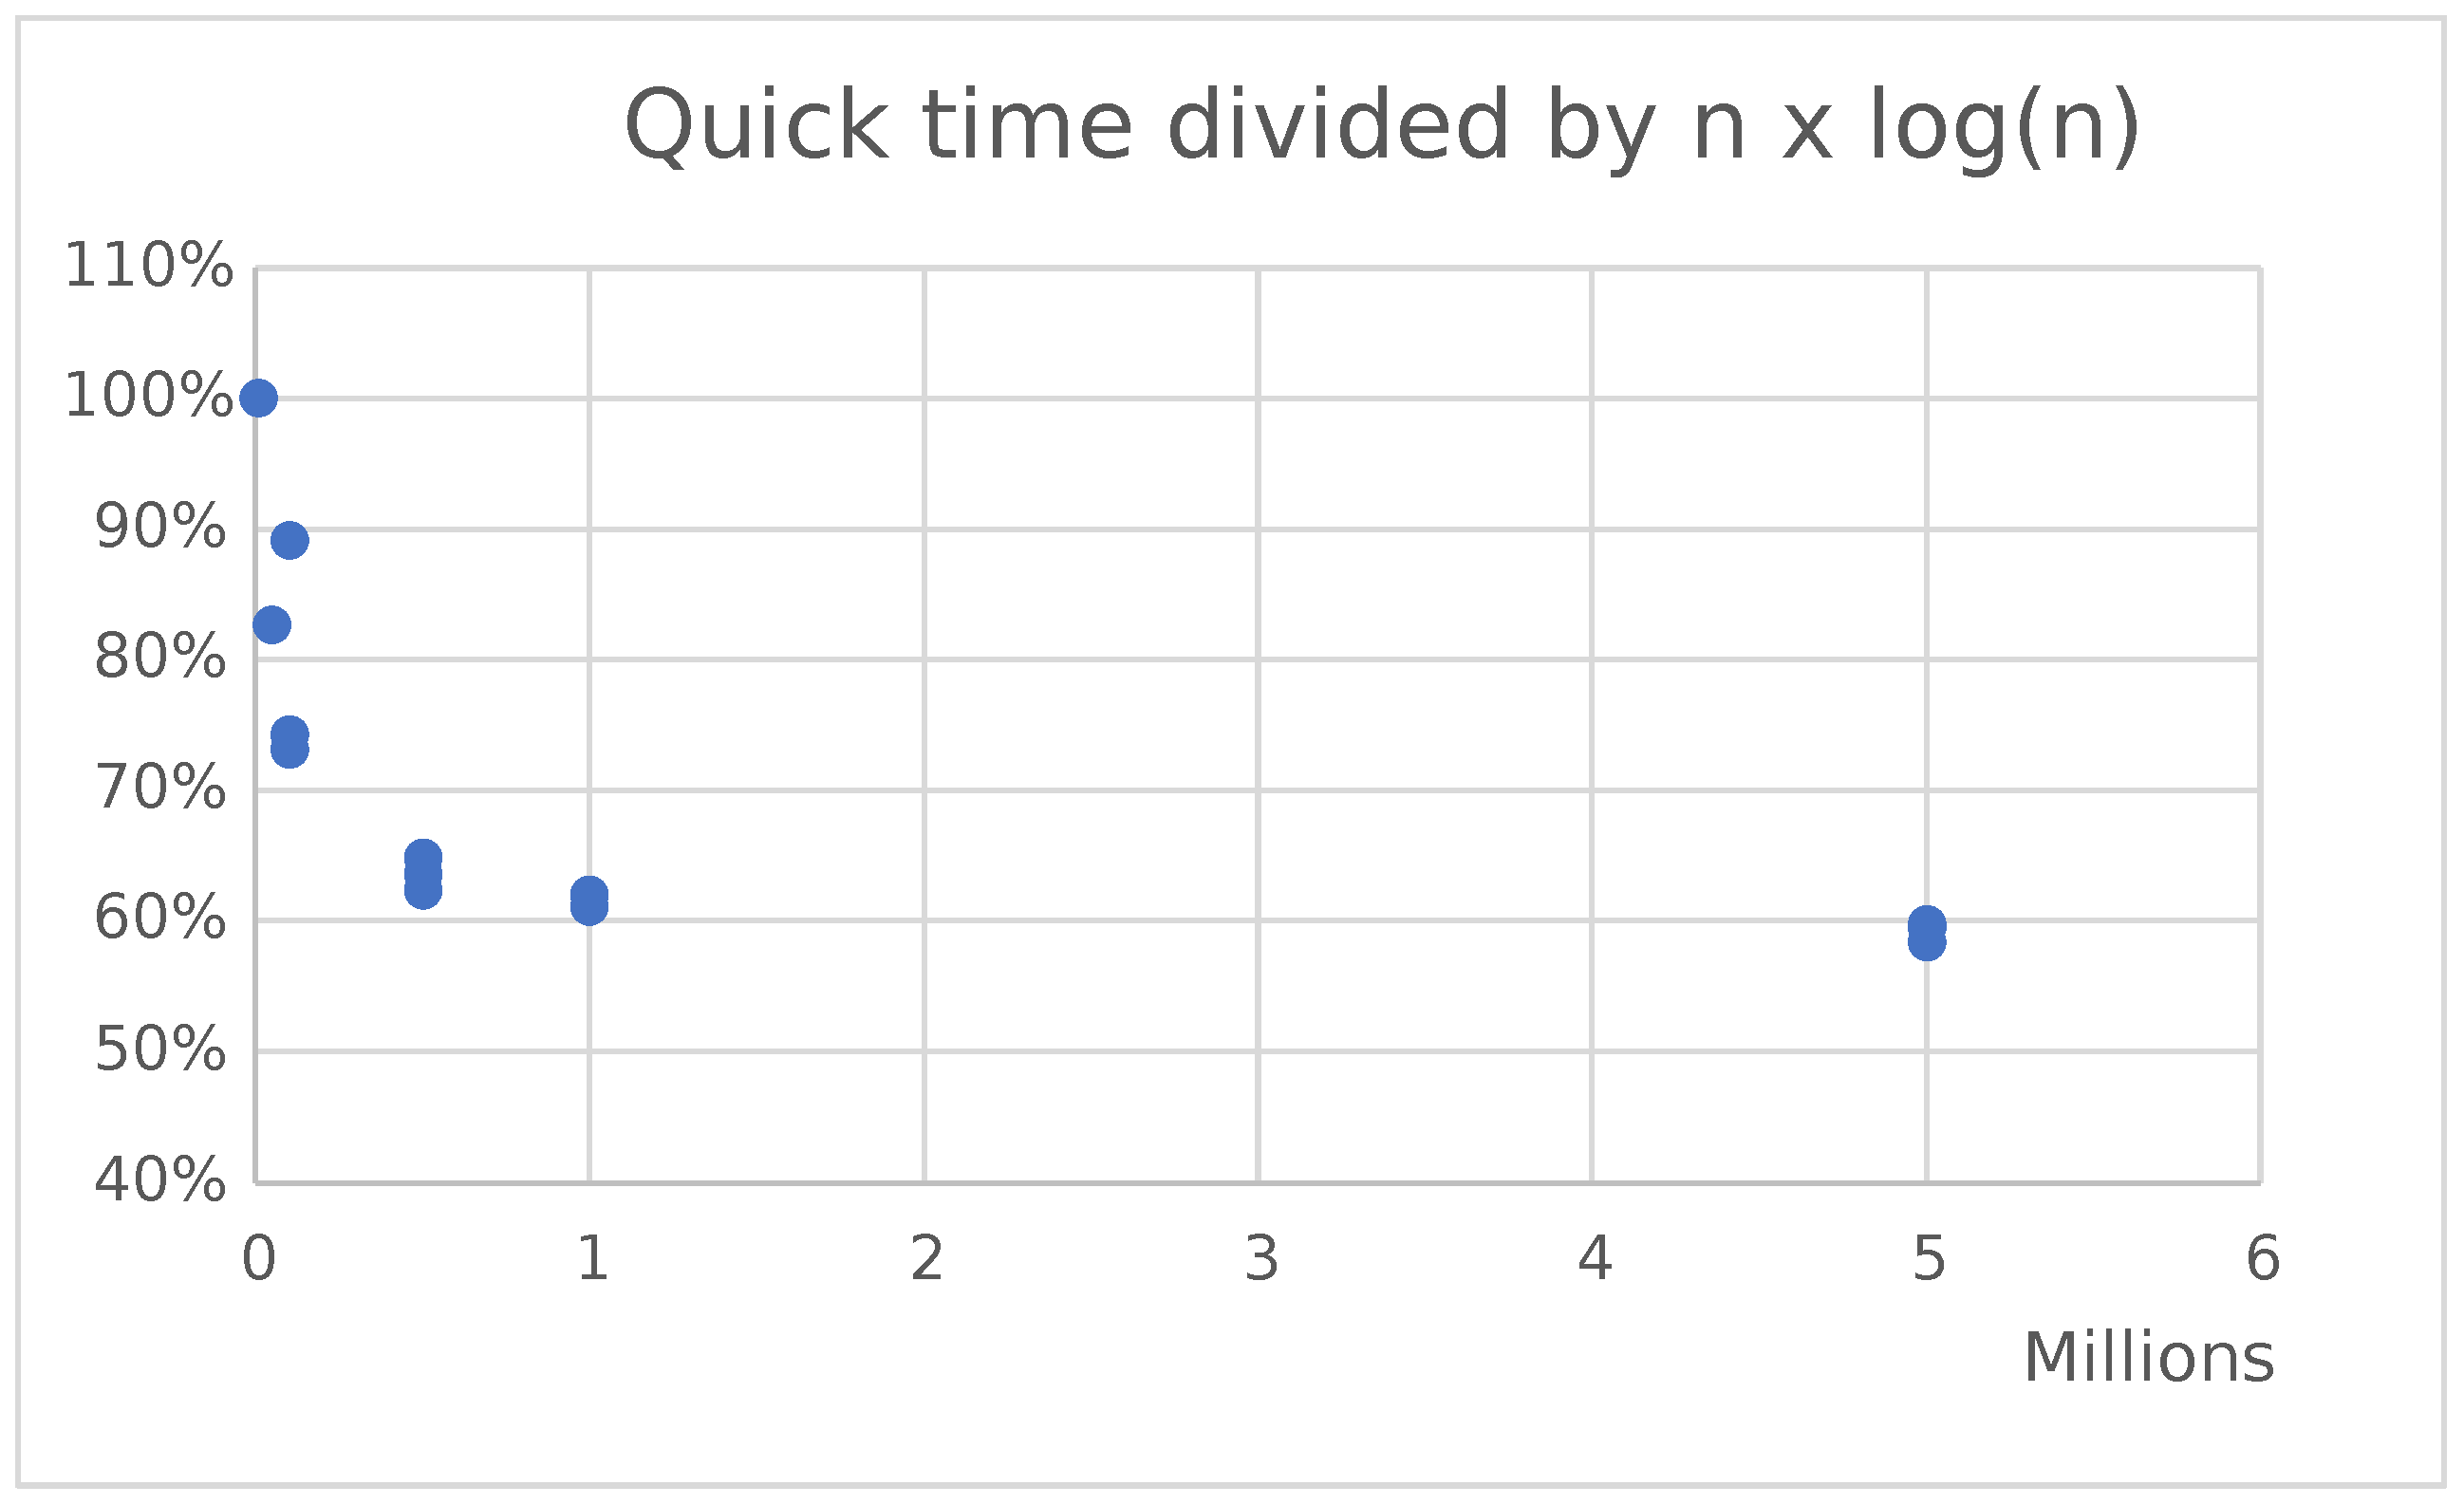
\includegraphics[width=185px]{assets/quickSort.eps}
				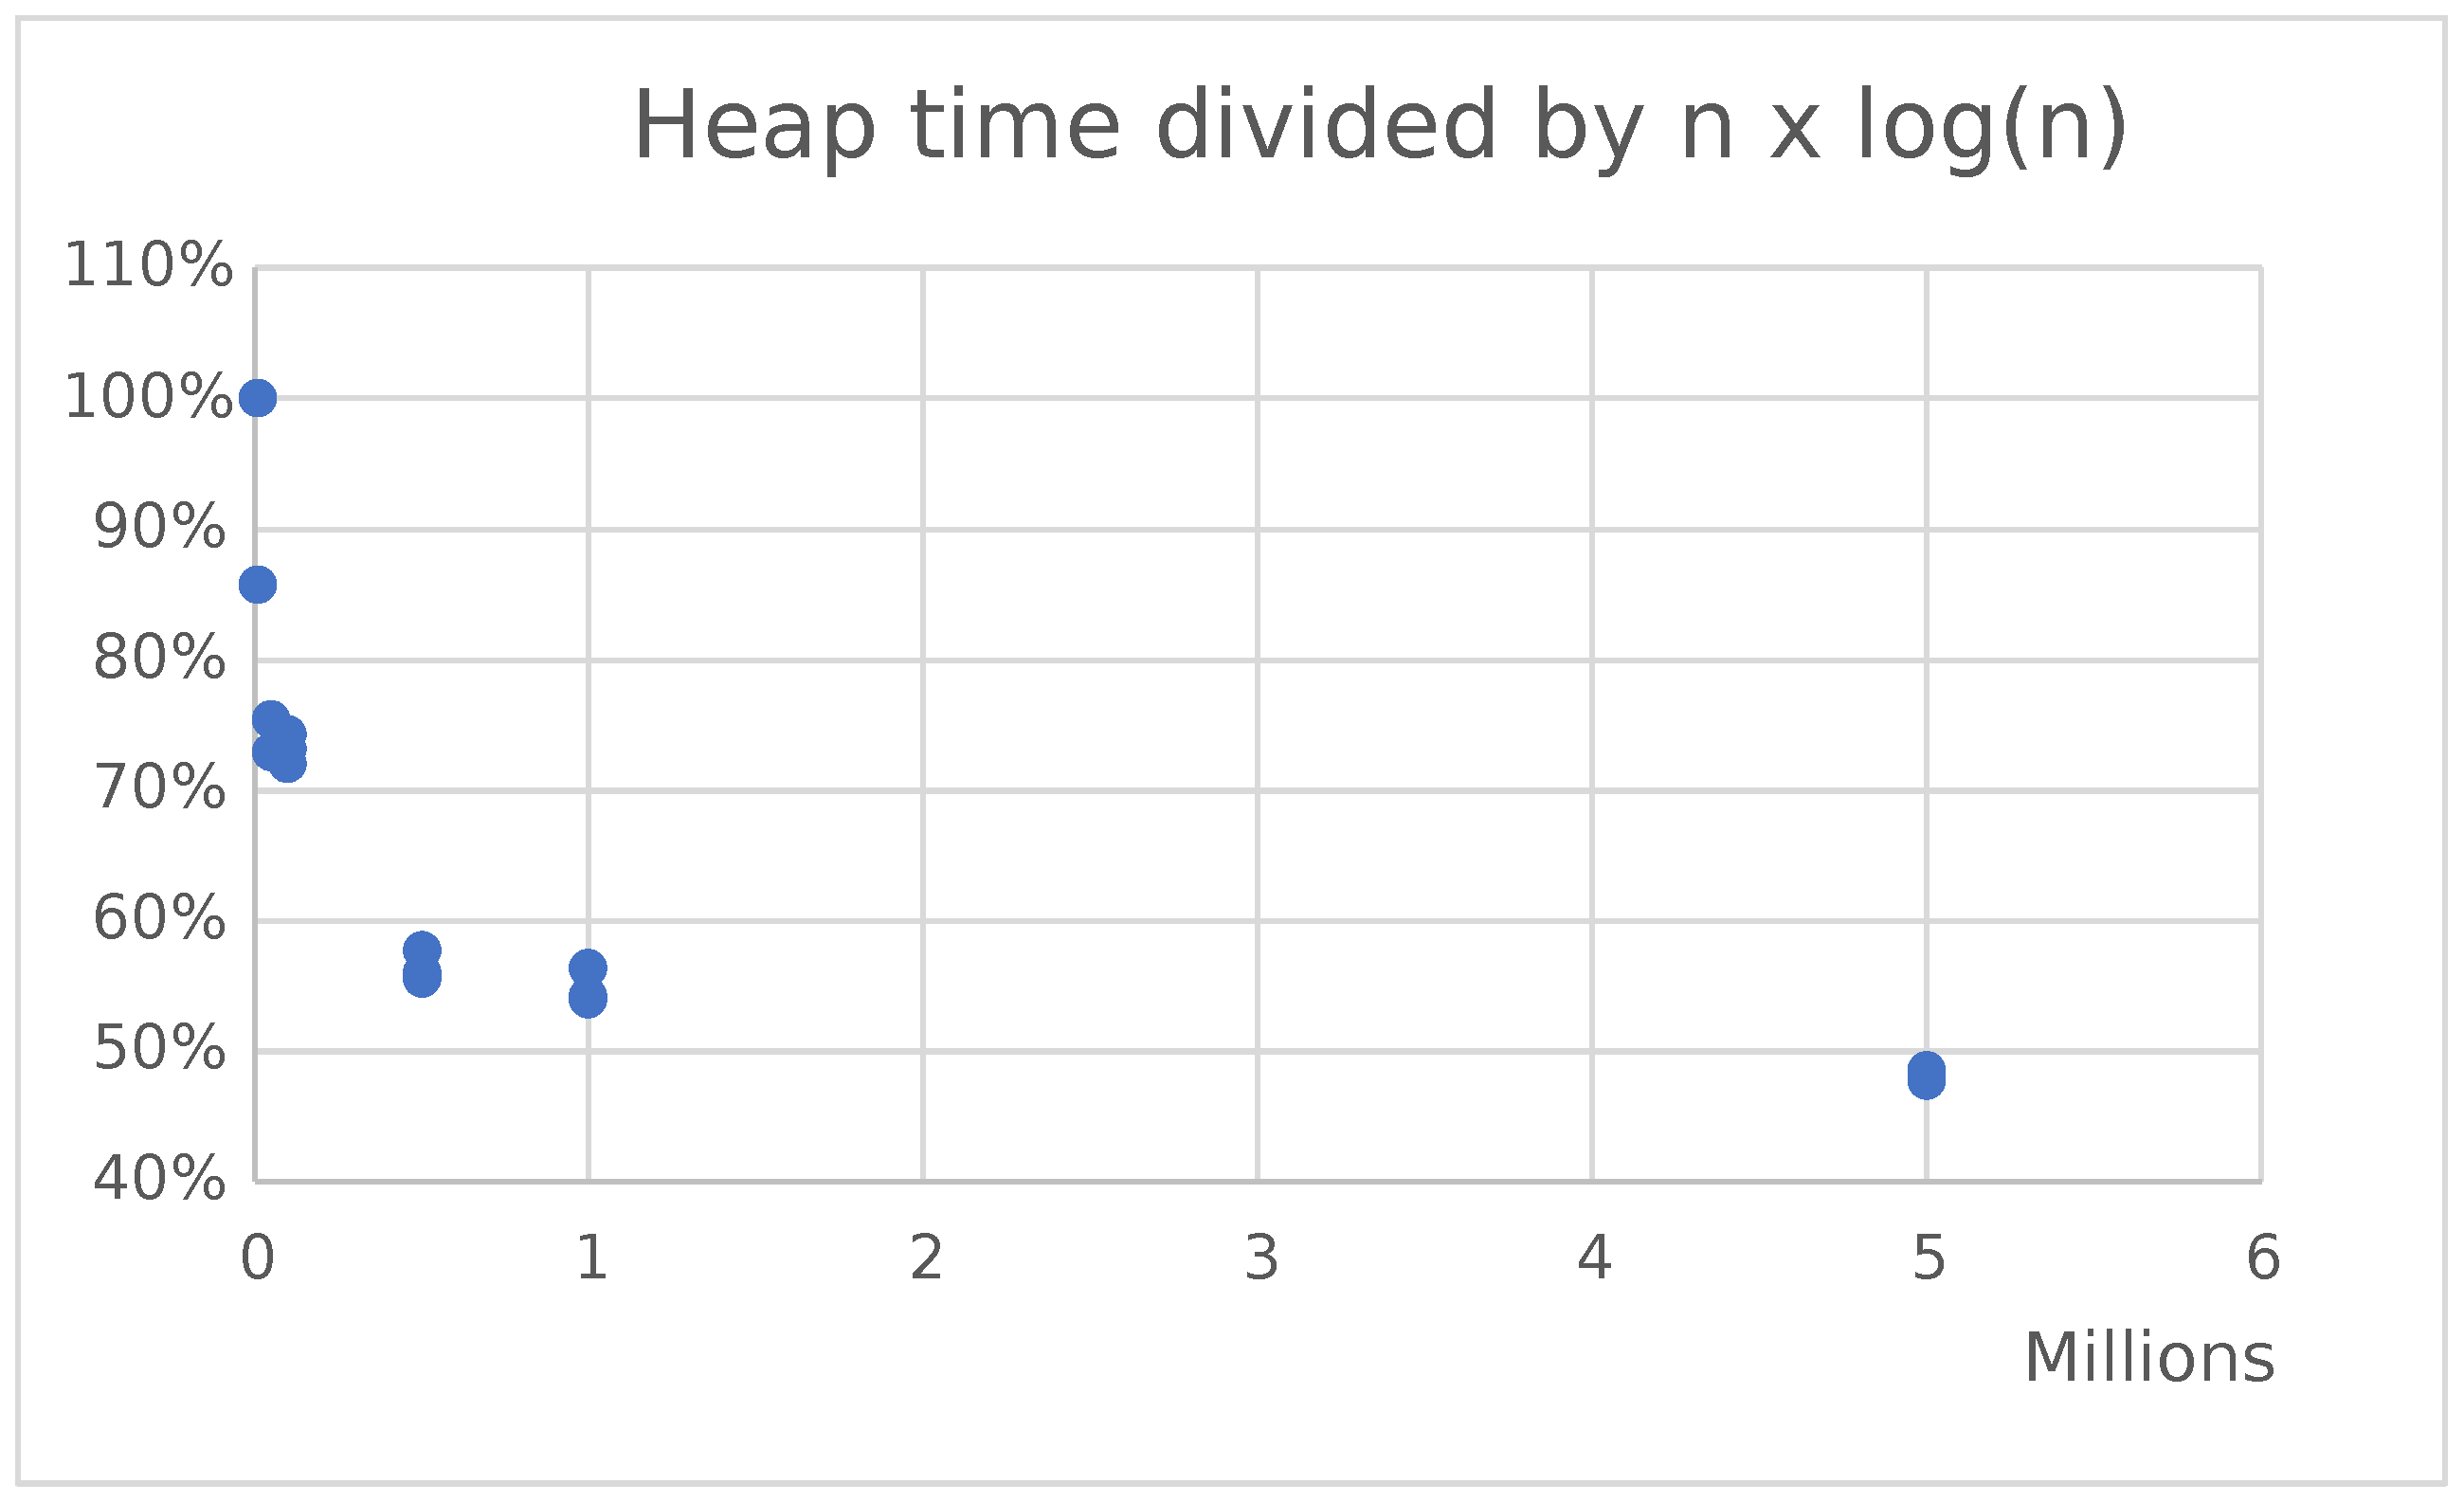
\includegraphics[width=185px]{assets/heapSort.eps}
				\caption{Graphs over the expected constant from dividing time with the sorting algorithms Big O notation}
				\label{fig:runTime}
			\end{figure}	
			This growth rate can be confirmed, by dividing the run time by the number of coordinates inserted into the growth rate function. It can then be seen in the three graphs \ref{fig:runTime}, that in the start it fluctuates, due to overhead having more influence and chance of more or less optimal coordinate files, but then stabilizes at a constant. This constant confirms that the implementations run time match the expected run time of big O notation.
		\subsection{Sorting times in relation to number of comparisons}
			With the Big O notation being based on number of comparisons, it should be expected that the number of comparisons pr. second should be constant through the sorting algorithms.\\	
			In the graph \ref{fig:MCIPS} is the number of million comparisons per second (MCIPS) graphed for each of the 3 algorithm. The 3 algorithm MCIPS is graphed when performened on 10,000, 100,000, and 1,000,000 coordinates respectively. It can here be seen that a constant was not reached, and the fluctuations was high.\\
			In the insertion sort algorithm the MCIPS was substantially lower. The is most likely due to a larger amount of time, was used to move data around rather than comparing data.\\
			For heap sort and quicksort the MCIPS seemed to still be growing. It should be expected on large enough sets of coordinate the MCIPS should reach a constant MCIPS.\\
			It can be seen that the second test for heap sort was an outlier. This is likely due to a random set of coordinates which required little moving of data.
			\begin{figure}[h]
				\centering
				\includegraphics[width=300px]{assets/MCIPS.eps}
				\caption{Number of millions comparisons per second on the $y$ axis and the algorithm on $x$ axis. The algorithms was ran with input size of 10,000, 100,000, and 1,000,000 coordinates }
				\label{fig:MCIPS}
			\end{figure}	
	\section{Conclusion}
	As seen in the benchmark the heap sort algorithm is the fastest, but that comes at a cost of complexity. As a measure of complexity the implementations length of readability can be used.\\
		The insertion sort is the least complex with around 20 lines of code and easy readability, but has the fastest growth rate.\\
		Heap sort was the fastest sorting algorithm but also took around 80 lines of code and require an understandment of the heap structure in order to read and understand the code.\\
		In the middle between heap sort and insertion sort is quicksort. The implementation required around 50 lines of code and its recursive nature make it easier to read and understand. Quicksort had a run time near heap sort, but on average will run a little slower.\\
\end{document}
